\documentclass[12pt, a4paper]{article}
\usepackage{graphicx}
\usepackage{fourier}
\usepackage{indentfirst}

\title{\Huge Cloud Databases}
\author{\Large Leon Radó}
\date{\today}

\begin{document}

\maketitle
\begin{figure}[b]
    \centering
    
\includegraphics[width=0.8\linewidth]{images/STU-FIIT.png}
\end{figure}
\thispagestyle{empty}

\clearpage
\tableofcontents

\clearpage
\begin{abstract}
    The following article provides a brief overview of cloud computing, especially databases. Firstly, it describes the main principles of cloud databases, their differences from standard on-premises databases, and their options of implementation. Later, the reader will learn about the process of database search with the use of indexes. Afterward, this writing introduces different types of database systems, as well as the benefits, disadvantages, and concerns of cloud databases. In this section, essential properties of cloud databases, like cost-effectiveness, flexibility, accessibility, and maintenance are evaluated. In the end, it mentions the latest trends and future of cloud computing, like serverless databases and multi-cloud database solutions. After reading this paper, the reader will gain basic knowledge of database systems and understand the importance and rising popularity of cloud computing.\\\\
    \footnotesize{\textbf{Keywords: }\textit{database, cloud computing, relational database, nosql, cloud provider}}
\end{abstract}
\clearpage

\section{Introduction}
    A cloud database is a particular type of database that works just like a standard on-premise database system but differs by its type of placement. While traditional databases exist on physical servers, cloud databases operate in a cloud environment. That means the database system is not located in the business infrastructure, but instead, it is accessible via the cloud by a specific cloud service provider. \textit{Cloud computing has become the norm in today's computing world. This paradigm shift is looking for databases that are compatible in all respects.}\cite{03} Each of these two types has an advantage over the other in terms of cost-effectiveness, accessibility, performance, security, and many other important characteristics, so it is up to the business owner to choose the right option for the purpose and requirements of his business. \par In this article, I will mainly focus on the benefits and disadvantages that come with cloud databases to understand how these new types of databases work and what improvements they can offer to the world of data management.
\clearpage

\section{Cloud Database Implementation}
    There are two primary methods to implement a cloud database, the thing they have in common is the presence of a third-party cloud service provider. One of these options is operating the database on the cloud independently of the provider with the virtual machine. Another option is using the database as a service (DBaaS).
    
    \subsection{Virtual Machine Image}
        Providers allow users to create a virtual machine image to directly access a database stored on the cloud. This virtual machine includes the database software, operating system, and necessary configurations.\par The owner pays for the specific resources he needs, the cost is predictable and based on the resources and services he selects. This type of implementation requires manual and more demanding management but offers better control of the database and more options for customization.
    
    \subsection{Database as a Service}
        DBaaS is a more commonly used method to implement a cloud database. This service provides a database for the user through the Internet and includes hosting, setup, and management of the system, so the user doesn't have to worry about additional complex work related to maintaining a database. \textit{Enterprises may focus on their core competencies instead of having to maintain complex IT landscapes.}\cite{11}\par DBaaS most often follows a pay-as-you-go pricing method, which means the owner pays just for the resources utilized at the moment.
        \begin{figure}[b]
            \centering
            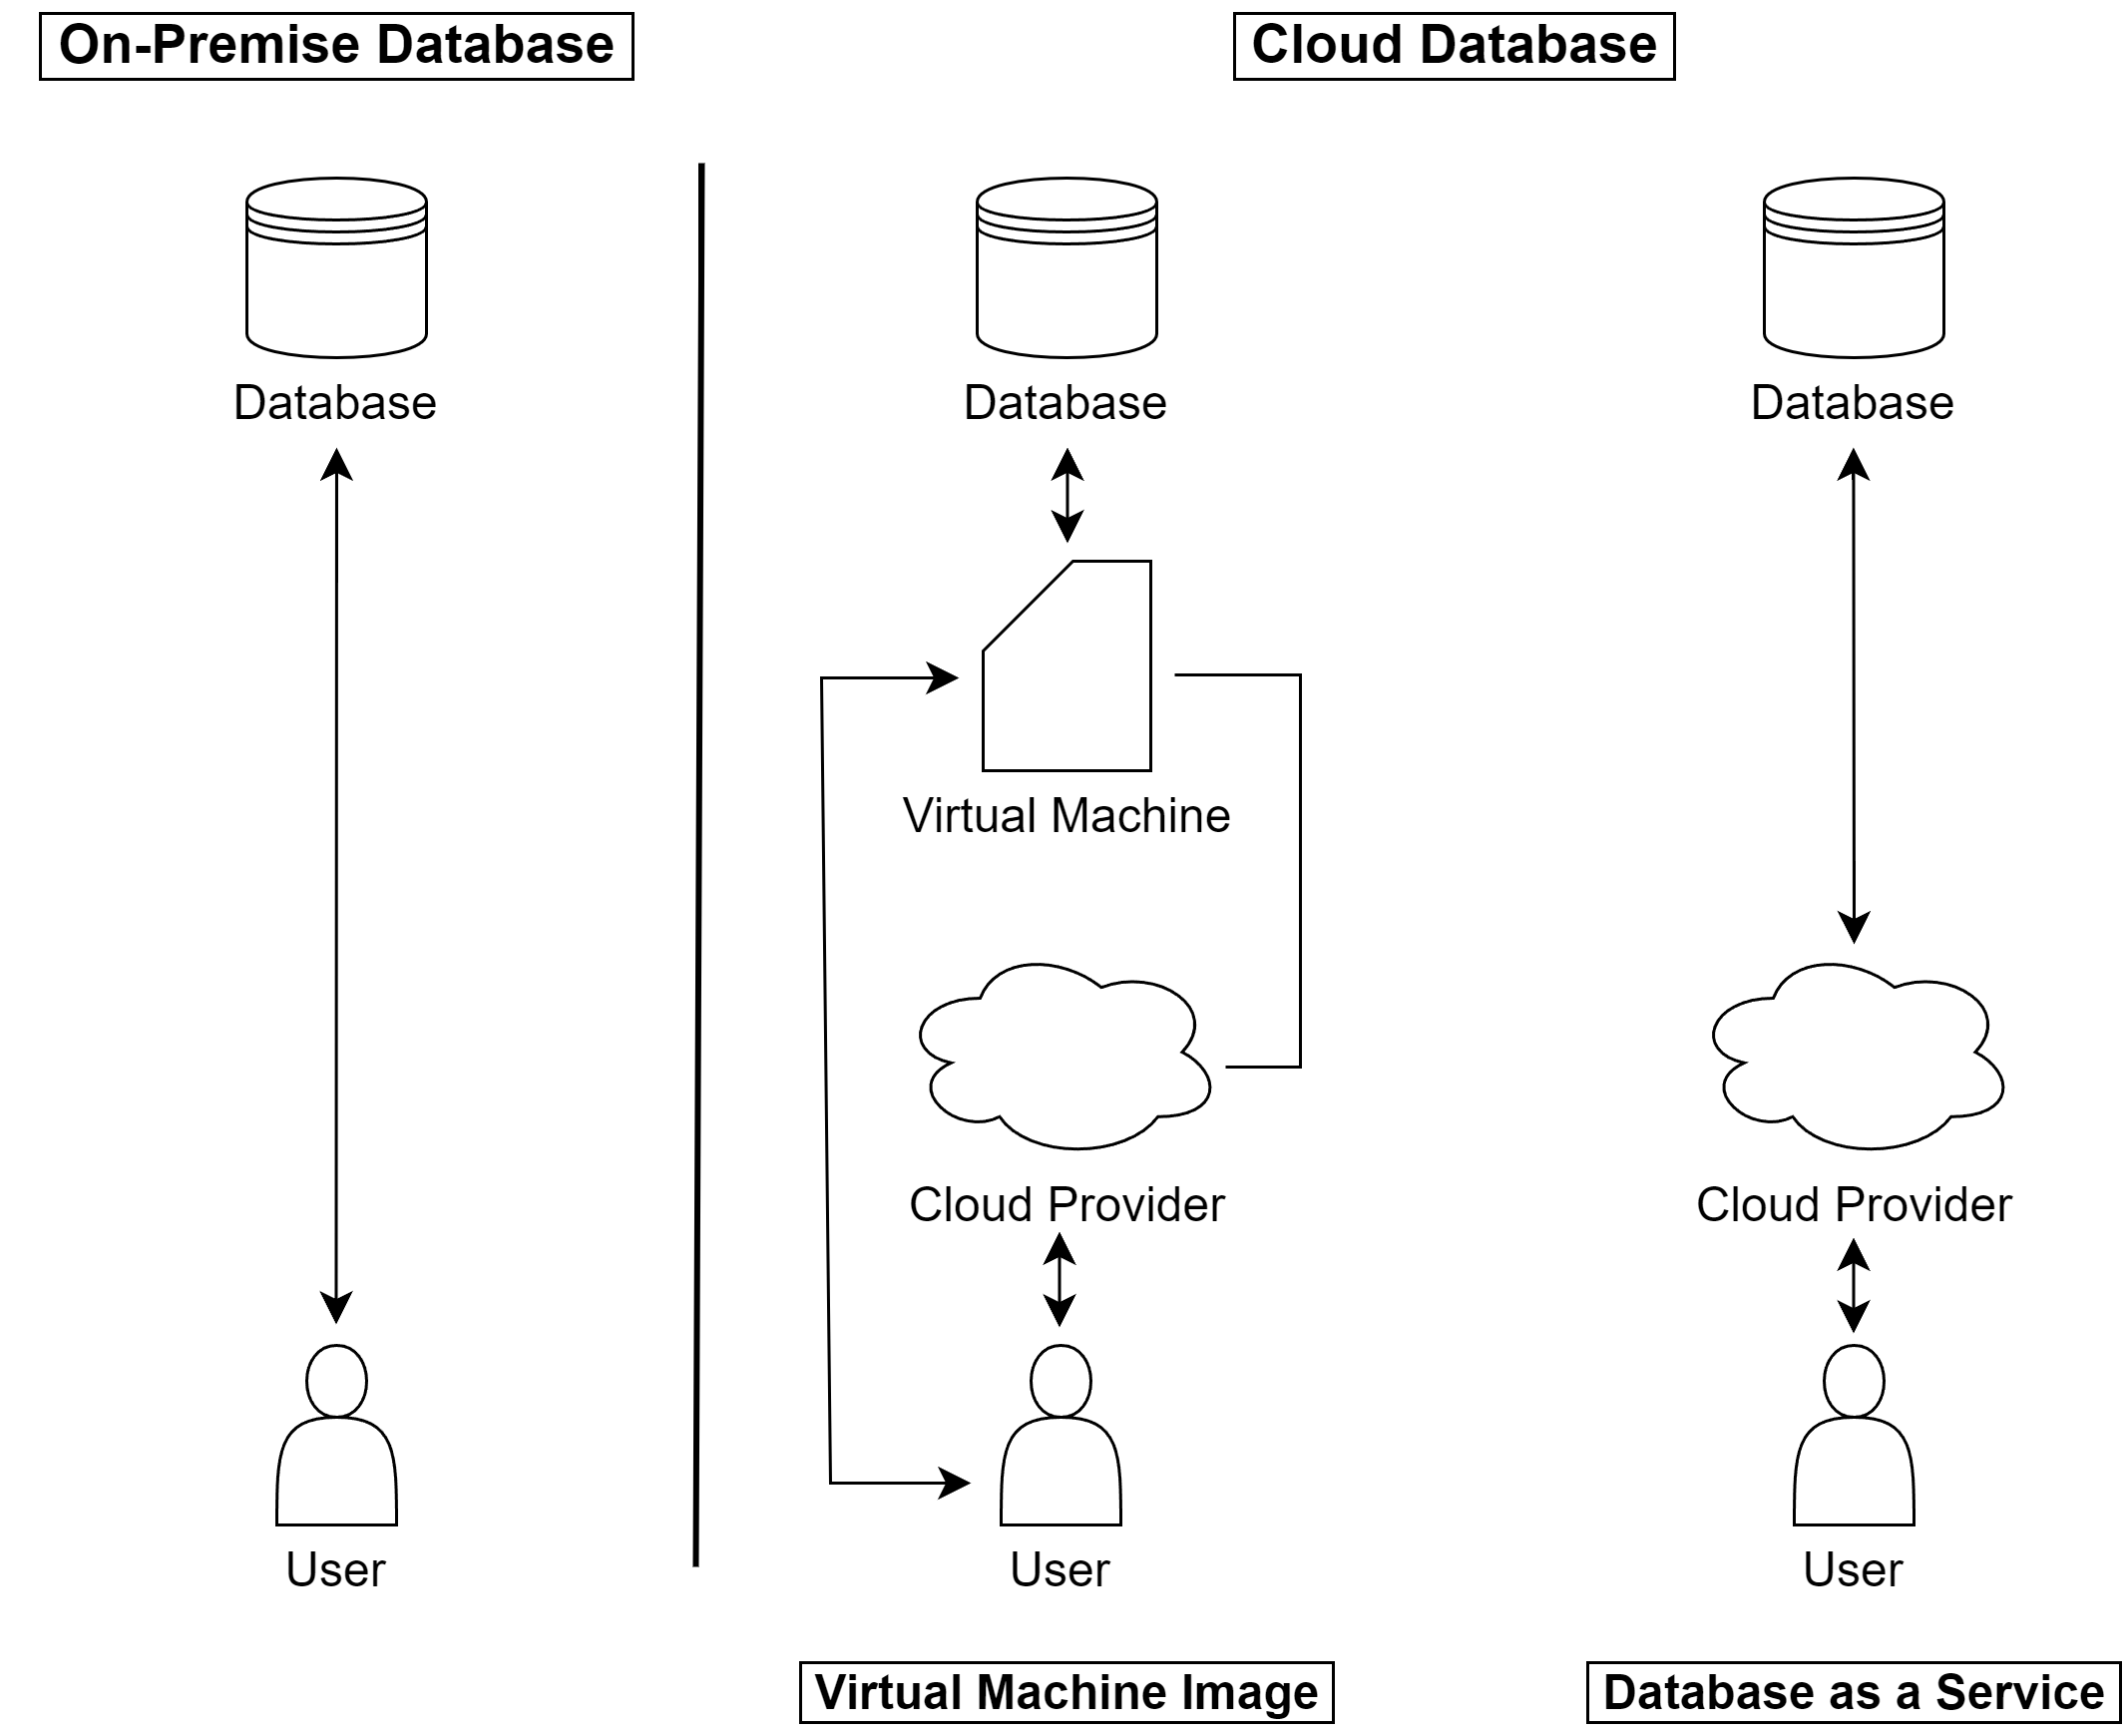
\includegraphics[width=1\linewidth]{images/onpremise-cloud.png}
            \caption{Comparison of Database Systems}
            \label{fig:comparison}
        \end{figure}
\clearpage

\section{Types of Cloud Databases}
    Just like standard on-premise databases, cloud databases can be divided into relational databases and non-relational, usually referred to as NoSQL databases. When choosing the right database it's important to consider the strengths, weaknesses, and use cases of both types.

    \subsection{Relational Databases}
        These databases store structured information organized into rows and columns, the structure of the data has to be defined in advance. Relation databases are typically used for applications with structured data, for example, transactional systems, and offer consistency and reliability, however, they are usually scaled vertically, which means they can be demanding on server resources like CPU and RAM.

    \subsection{NoSQL Databases}
        Non-relational databases are designed to work with a large amount of unstructured data, that is most often stored in key-value pairs without predefined format. This type of database is adequate for example for web applications that store a variety of information. \textit{NoSQL databases were born to meet performance needs, leaving other details like atomicity in the background.}\cite{06}\\
        \begin{figure}[h]
            \centering
            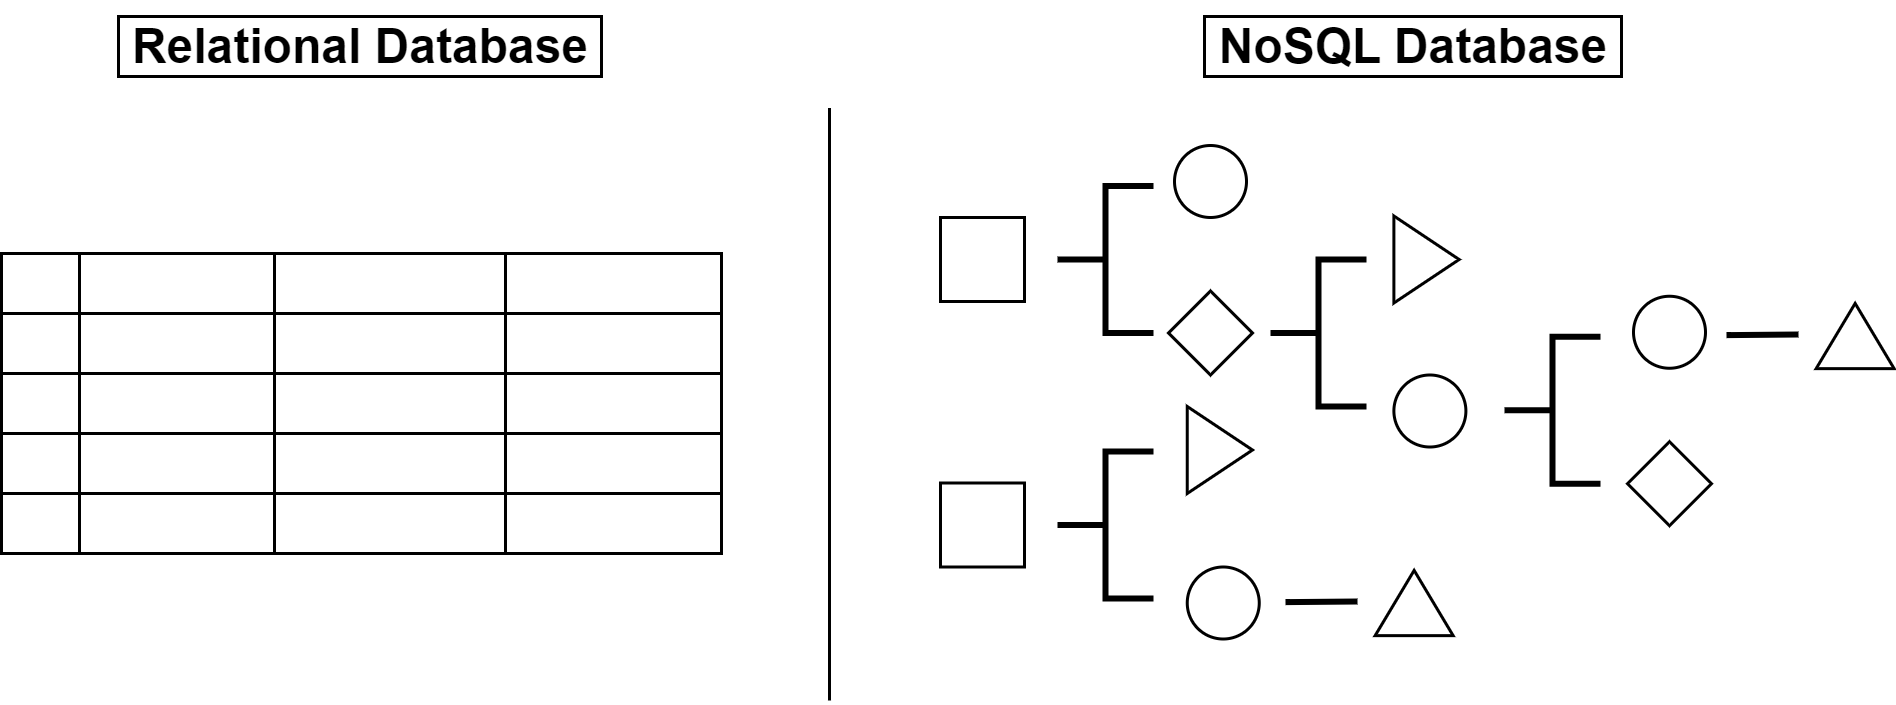
\includegraphics[width=1\linewidth]{images/relational-nosql.png}
            \caption{Structure of Relational and NoSQL Database}
            \label{fig:structure}
        \end{figure}
\clearpage

\section{Database Search}
    In order to retrieve information from a database, the corresponding database has to go through the process of database search. After the user provides a search query related to the information he wants to extract, the database starts searching for the relevant data. 
    
    \subsection{Indexing}
        Comparing every record stored in the database to the specific search query can be really time-consuming, especially for larger database systems. However, this problem can be effectively resolved by using indexes. \textit{To gain the speed benefits of indexing at retrieval time, the indexing algorithm is proposed and an index table is built by this algorithm in advance.}\cite{15}\par Indexing ensures that each record in the database obtains a new key-value pair data structure, where the key is a column with the content that might be potentially queried, and the value is a reference to the exact location in the database.
    
    \subsection{Query Language}
        When the user needs to extract information from a database, it is necessary for him to use language compatible with that database. This language will mostly depend on whether the database is relational or non-relational but also on the respective database provider.\par The following example shows a search query for data from the 'books' category by the author 'Joel Lord' from the relational and NoSQL databases, respectively.\\

    \begin{figure}[h]
        \centering
        \fbox{
\includegraphics[width=0.9\linewidth]{images/sql.png}}
        \caption{Search Query in SQL (Structured Query Language)\cite{101}}
        \label{fig:sql}
    \end{figure}

    \begin{figure}[h]
        \centering
        \fbox{
\includegraphics[width=0.9\linewidth]{images/mongodb.png}}
        \caption{Search Query in MongoDB Query Language\cite{101}}
        \label{fig:mongodb}
    \end{figure}
\clearpage

\section{Benefits of Cloud Databases}
    \subsection{Accessibility}
        Accessing a cloud database isn't limited by geographical location and can be done from anywhere with a stable Internet connection. This feature is especially useful for organizations that need access to the database from different locations.
    
    \subsection{Scalability}
        Cloud databases are designed to be highly scalable, which means they can process vast amounts of data with great performance. They also support a large amount of users and applications without the need for additional hardware installation.

    \subsection{Cost-Efficiency}
        Because of the missing need for investment into hardware installation, cloud databases are more cost-efficient. \textit{Cloud computing can provide almost immediate access to hardware resources, with no upfront capital investments for users, leading to a faster time to market in many businesses.}\cite{12}\par The pay-as-you-go model also gives assurance that enterprises pay for the resources, they actually utilize. However, it's always important to regularly analyze and optimize the resources to avoid unnecessary overspending.
        
    \subsection{Managed Services}
        Cloud databases are in most cases managed by cloud providers, which results in enhanced reliability because of their high level of expertise in this field. Owners don't have to worry about tasks like database administration, patching, and maintenance.
        
    \subsection{Disaster Recovery}
        Cloud providers offer services to automatically backup and recover the data in need, which results in a decreased risk of data loss in case of natural disaster or hardware malfunction. \textit{Since all the data is stored in the cloud, backing it up and restoring the same is relatively much easier than storing the same on a physical device.}\cite{13}
\clearpage

\section{Disadvantages and Concerns of Cloud Databases}
    \subsection{Data Security}
        Despite the fact cloud databases have high security standards, there is always a risk of information theft and unauthorized access. \textit{The chances that the host company may violate the privacy of its customers and access data without permission, make some potential customers worried.}\cite{02} Since the data aren't stored locally, the owners need to reconsider their choice of storing sensitive information.

    \subsection{Limited Control}
        These types of databases are almost fully managed by a third-party provider, which can be unsuitable for businesses with special requirements because they aren't aware of how their data are accessed and managed. Options for customization are also very limited.
        
    \subsection{Network Dependency}
        Cloud databases rely on the Internet connection. This can be really problematic during network outages or other associated issues, especially for applications requiring low-latency real-time response.\par Furthermore, this type of service is always prone to serious malfunctions and interruptions. \textit{Even the best cloud service providers run into this kind of trouble, in spite of keeping up high standards of maintenance.}\cite{14}
        
    \subsection{Vendor Lock-In}
        Organizations that began to use a cloud database are heavily dependent on the particular cloud provider. Migrating to another cloud database or an on-premise database in the future can be very difficult and expensive.
    
    \begin{table}[t]
        \centering
        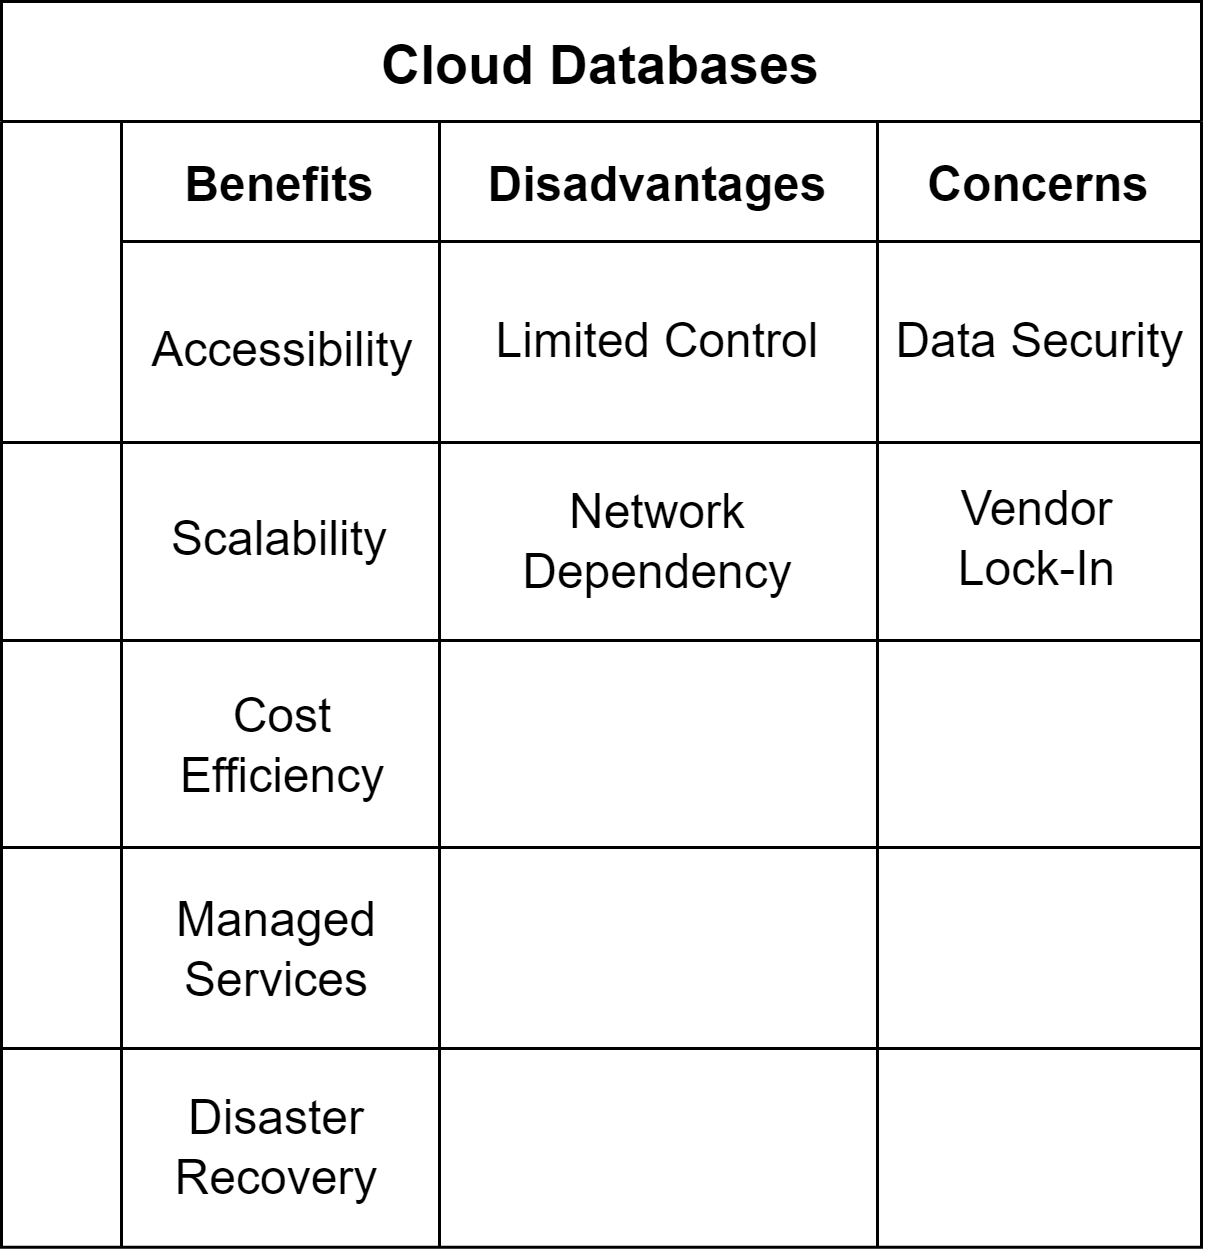
\includegraphics[width=0.65\linewidth]{images/benefits.png}
        \caption{Benefits, Disadvantages, and Concerns of Cloud Databases}
        \label{tab:benefits}
    \end{table}
\clearpage

\section{The Latest Trends in Cloud Databases}
    In the last few years, it has been possible to observe a high increase in the number of organizations transferring their data to the cloud. This transition led to the latest innovations and further development in this area. \textit{Advances in cloud computing technologies have changed the scene now and computing is being offered as a service over the internet.}\cite{09}
    
    \subsection{Serverless Databases}
        A serverless database is a type of cloud database that doesn't require any additional management on the server side from the user. These databases are automatically scaled, meaning the storage resources are automatically allocated and scaled up and down based on the current demand. Users can see information about the number of reads and writes and the size of utilized resources.
    
    \subsection{Multi-Cloud Database Solutions}
        Many enterprises utilize cloud databases by at least two different providers. This strategy is referred to as a multi-cloud database solution, and although it has its challenges, it comes with significant security improvements. \textit{The same tasks are performed on multiple clouds and their results are compared thereby the user can be assured of the integrity of the data.}\cite{17}\par With the implementation of this architecture, users are able to choose what data they want to store in each database as a result of not being dependent on one provider. This method also lowers the risk of potential vendor lock-in, and in case of natural disasters or service outages, businesses can rely on other providers.
        \begin{figure}[ht]
            \centering
            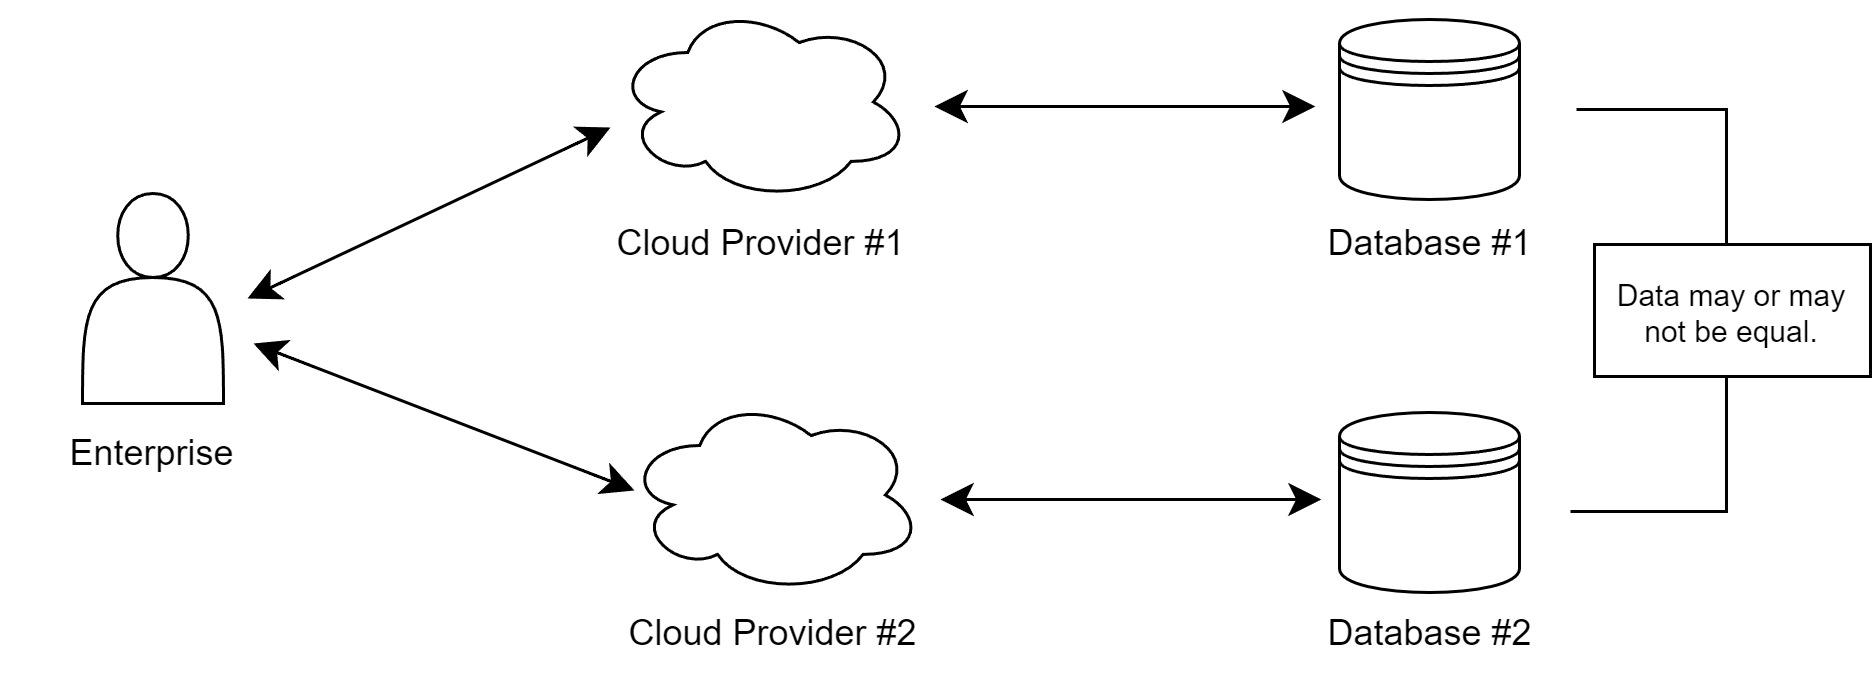
\includegraphics[width=1\linewidth]{images/multicloud.png}
            \caption{Multi-Cloud Architecture}
            \label{fig:multicloud}
        \end{figure}
        
    \subsection{AI in Database Management}
        With the expansion of artificial intelligence in recent years, apart from everything else, it has also become a tool to enhance the database management process. Machine learning algorithms help to boost performance, predict analytics, and perform automated maintenance tasks. Last but not least, embedding natural language processing (NLP) for querying allows users to query for data by using human language.
\clearpage

\section{Conclusion}
    To sum up, in these times, we are experiencing a significant shift in movement towards cloud computing and databases. \textit{The rise of cloud computing opens a whole new future for the information technology area. However, open systems and shared resources give place to many security challenges, making security one of the main obstacles to the deployment of cloud computing technologies.}\cite{05}\par This paper introduced various cloud database systems and their implementation process and later compared their benefits and drawbacks. We can identify cloud databases as cost-effective, fast, scalable, and easier to utilize but on the other hand also less secure, and dependent on the network connection and particular cloud provider.\par Although these disadvantages can be partially minimized by multi-cloud architecture, a cloud database still might not be the optimal solution for every occasion. It's always on the organization to choose the best option for the type and specifications of the stored data. However, cloud databases are becoming more and more widespread every moment and this rise doesn't seem to stop anytime soon.
\clearpage

\bibliographystyle{unsrt}
\bibliography{refs}

\end{document}
